% PFTF_alpha_소개.tex -- 대학원생용 쉬운 설명서
% Canonical rule: 논문생성규칙.md 명령 2.
% Target: graduate readers, explained with Korean high-school mathematics.
% Final PDF requested explicitly by the user on 2026-08-04.
\documentclass[11pt,a4paper]{article}

\usepackage[margin=24mm]{geometry}
\usepackage{kotex}
\usepackage{amsmath,amssymb}
\usepackage{graphicx}
\usepackage{booktabs}
\usepackage{tabularx}
\usepackage{array}
\usepackage{xcolor}
\usepackage{setspace}
\usepackage{enumitem}
\usepackage[section]{placeins}
\usepackage[labelfont=bf,labelsep=period]{caption}
\usepackage{fancyhdr}
\usepackage[hidelinks]{hyperref}

\graphicspath{{draft/pics/}{pics/}}
\onehalfspacing
\setlength{\parskip}{3pt}
\setlength{\parindent}{1em}
\setlength{\emergencystretch}{2em}
\setlength{\headheight}{14pt}
\setlist[itemize]{leftmargin=1.5em,itemsep=2pt,topsep=3pt}
\setlist[enumerate]{leftmargin=1.7em,itemsep=3pt,topsep=3pt}
\renewcommand{\arraystretch}{1.18}

\definecolor{deepblue}{HTML}{244B74}
\definecolor{softblue}{HTML}{EAF2F8}
\definecolor{softgreen}{HTML}{E9F7EF}
\definecolor{softred}{HTML}{FDEDEC}
\newcommand{\yes}{\textcolor{deepblue}{\textbf{지지됨}}}
\newcommand{\no}{\textcolor{red!65!black}{\textbf{지지되지 않음}}}
\newcommand{\code}[1]{\texttt{#1}}

\pagestyle{fancy}
\fancyhf{}
\fancyhead[R]{\small PFTF-alpha 쉬운 설명서}
\fancyfoot[C]{\thepage}
\renewcommand{\headrulewidth}{0.4pt}

\hypersetup{
  pdftitle={PFTF-alpha 연구를 쉽게 이해하는 안내서},
  pdfauthor={},
  pdfsubject={Alpha shape, PFTF hypothesis testing, and layer-first reconstruction},
  pdfkeywords={alpha shape, point cloud, PFTF, two layer, S3DIS}
}

\title{\textbf{PFTF-alpha 연구를 쉽게 이해하는 안내서}\\[5pt]
\large ``더 좋은 $\alpha$ 찾기''에서 ``연결을 먼저 제한하기''까지\\[7pt]
\normalsize 대학원생을 위한 설명서이지만, 수학은 고등학생 눈높이로}
\author{}
\date{2026년 8월 4일}

\begin{document}
\maketitle
\thispagestyle{fancy}

\begin{abstract}
\noindent
3D 스캐너가 주는 것은 매끈한 표면이 아니라 흩어진 점들의 모임이다. 이 점들을
삼각형으로 이어 표면을 만들 때, convex hull은 너무 볼록하고 alpha shape은
더 섬세하지만 $\alpha$ 값을 정하기가 어렵다. 이 프로젝트는 처음에 PFTF의
방향 정보로 장소마다 더 알맞은 ``거리 자'' 또는 좌표 변환을 만들면 이 문제를
해결할 수 있는지 물었다. 엄격한 실험 결과, PFTF/local-SPD가 기존 anisotropic
alpha보다 낫다는 주장은 지지되지 않았다. 그러나 연구는 여기서 끝나지 않았다.
서로 떨어진 두 표면에서는 $\alpha$를 더 잘 고르는 것보다, 먼저 두 층을 나누고
각 층 안에서만 연결하게 하는 것이 훨씬 효과적이었다. 144개 합성 확인 사례와
서로 다른 건물의 S3DIS 63개 방에서 이 좁지만 분명한 양성 결과가 재현되었다.
이 문서는 원래 가설, 실패한 경로, two-layer 전환, 검증 수치와 한계를 한 흐름으로
최대한 쉽게 설명한다.
\end{abstract}

\tableofcontents
\newpage

\section{먼저 결론부터: 이 프로젝트는 무엇을 알아냈나?}

긴 설명을 읽기 전에 결론을 세 줄로 줄이면 다음과 같다.

\begin{enumerate}
  \item \textbf{Alpha shape은 convex hull보다 복잡한 모양을 잘 표현하지만,
  $\alpha$ 선택은 실제로 어렵다.}
  \item \textbf{PFTF를 local-SPD 거리나 좌표 변환에 연결한 시도는 수학적으로
  흥미로운 구성은 만들었지만, 더 좋은 복원 성능을 보이지 못했다.}
  \item \textbf{서로 분리된 두 표면에서는 더 좋은 $\alpha$를 찾는 대신 두 층을
  먼저 나누고 층별로 연결하는 방법이 강한 양성 결과를 냈다.}
\end{enumerate}

따라서 이 프로젝트의 최종 메시지는 ``PFTF가 최적의 $\alpha$를 예측했다''가
아니다. 더 정확한 문장은 다음과 같다.

\begin{quote}
\textbf{충분히 평면에 가깝고, 넓게 겹치며, 서로 간격이 큰 두 표면에서는
관측 좌표만으로 두 층을 먼저 구분하고 각 층 안에서만 연결하는 것이
anisotropic/weighted alpha보다 정확하고 topology도 안전했다.}
\end{quote}

여기서 중요한 말은 \emph{충분히}, \emph{두 표면}, \emph{간격이 큰}이다.
아무 점군에나 통하는 만능 해법이 아니라, 조건이 명확한 특수 문제를 제대로
해결한 결과다.

\section{출발점: 점군에서 표면을 어떻게 만드는가?}

\subsection{점군은 ``3D 별자리''다}

3D 스캐너나 LiDAR가 물체를 측정하면 컴퓨터에는 점들의 좌표
$(x,y,z)$가 저장된다. 이것을 \textbf{점군}\footnote{점군(point cloud)은
공간에 흩어진 점의 모임이다. 각 점은 위치만 가질 수도 있고, 색·세기·법선 같은
부가 정보를 함께 가질 수도 있다. 본 연구의 핵심 후보는 결합된 XYZ 좌표만 받는다.}
이라고 한다. 점군은 별자리와 비슷하다. 점은 보이지만, 어느 점을 어느 점과
이어야 하는지는 적혀 있지 않다.

컴퓨터가 해야 할 일은 점들을 삼각형으로 이어 \textbf{메시}\footnote{메시(mesh)는
삼각형이나 사각형을 이어 만든 표면이다. 3D 프린팅, 게임, 시뮬레이션에서 물체의
껍질을 표현할 때 널리 쓴다.}를 만드는 것이다. 이때 두 종류의 실수가 생긴다.

\begin{itemize}
  \item 너무 적게 이으면 표면에 구멍이 난다.
  \item 너무 많이 이으면 원래 떨어져 있어야 할 부분 사이에 거짓 다리가 생긴다.
\end{itemize}

\subsection{Convex hull은 안전하지만 너무 단순하다}

Convex hull은 점군 전체를 고무막으로 감싼 모양이라고 생각하면 된다.
구현이 단순하고 항상 하나의 볼록한 껍질을 주지만, 오목한 홈이나 떨어진 부품을
표현하지 못한다. U자 모양을 고무막으로 감싸면 가운데 빈 곳까지 막혀 버리는 것과
같다.

\subsection{Alpha shape은 더 섬세하다}

Alpha shape은 Delaunay triangulation\footnote{Delaunay triangulation은
점들을 가능한 한 ``너무 뾰족하지 않은'' 삼각형 또는 사면체로 연결하는 대표적인
기하학적 밑그림이다. Alpha complex는 이 밑그림에서 일부 cell만 남기고,
alpha shape은 그 결과의 바깥 경계를 뜻한다. 일상 설명에서는 둘을 넓게
``alpha shape 방법''이라고 부르기도 한다.}에서 필요한 연결만 고른다.

각 선·삼각형·사면체에는 그것을 감쌀 수 있는 빈 공의 크기와 관련된 점수가 있다.
그 점수가 $\alpha$보다 작을 때만 그 연결을 남긴다고 생각하면 된다.

\begin{itemize}
  \item $\alpha$가 작으면 짧고 매우 가까운 연결만 남아 구멍이 많아진다.
  \item $\alpha$가 커지면 더 긴 연결까지 들어와 구멍이 메워진다.
  \item 너무 커지면 떨어진 부분도 붙고, 결국 convex hull에 가까워진다.
\end{itemize}

그래서 alpha shape은 convex hull보다 오목한 경계와 분리된 성분을 잘 표현한다.
대신 ``얼마나 크게 연결할까?''라는 손잡이 $\alpha$를 정해야 한다.

\section{왜 alpha 찾기가 애매한가?}

\subsection{좋은 값이 장소마다 다르다}

실제 점군은 밀도가 고르지 않다. 센서 가까운 곳은 점이 촘촘하고, 가려진 곳이나
비스듬한 곳은 성기다. 촘촘한 곳에 맞춘 작은 $\alpha$는 성긴 곳에 구멍을 만들고,
성긴 곳에 맞춘 큰 $\alpha$는 촘촘한 곳을 과도하게 붙인다.

즉 하나의 전역 $\alpha$로는 서로 다른 지역의 요구를 동시에 맞추기 어렵다.
더구나 alpha complex는 $\alpha$가 조금씩 변할 때 매 순간 연속적으로 바뀌는 것이
아니라, Delaunay cell의 유한한 임계값에서 계단처럼 바뀐다.
따라서 실제 선택은 ``마법의 실수 하나를 예측''하기보다 후보 임계값들을 평가하는
문제에 가깝다.\footnote{이 프로젝트의 구현은 내부에서 물리적 반지름의 제곱을
alpha 값으로 사용하고, 외부 표현에서 반지름과 제곱 반지름의 변환을 명시한다.
이 약속을 섞으면 숫자가 맞아 보여도 전혀 다른 scale을 비교하게 된다.}

\subsection{두 표면 문제에서는 scale만으로 부족하다}

책상과 천장처럼 서로 평행한 두 표면이 가까이 있다고 하자. 큰 $\alpha$를 쓰면
표면 안의 구멍은 잘 메워지지만 두 표면 사이에도 삼각형이나 사면체가 생긴다.
작은 $\alpha$를 쓰면 그 거짓 연결은 줄지만 각 표면 자체가 찢어진다.

이 상황에서 핵심 질문은 ``어느 정도로 멀리 이을까?''만이 아니다.
\textbf{``어떤 종류의 연결을 처음부터 허용할 것인가?''}가 더 중요하다.

\section{PFTF를 적용하려 했던 생각}

\subsection{PFTF의 원래 아이디어}

PFTF는 방향에 따라 달라지는 비용을 텐서장으로 모으고, source에서 receiver로
흐르는 관계를 표현하며, 신뢰할 수 있는 solver와 비교해 검증하는 일반 프레임워크다.
쉽게 말하면 다음 네 질문을 묻는다.

\begin{enumerate}
  \item 무엇이 비용을 만들어 내는가?
  \item 그 영향은 어디에서 어디로 흐르는가?
  \item 빠른 계산을 무엇과 비교해 믿을 것인가?
  \item 새 방법이 정말 필요한지 어떤 공정한 대조군으로 공격할 것인가?
\end{enumerate}

텐서\footnote{여기서는 방향 정보를 담은 행렬 정도로 이해하면 충분하다.
예를 들어 $x$ 방향은 짧게, $y$ 방향은 길게 재는 찌그러진 자를 숫자 표로
표현할 수 있다.}는 방향 정보를 한 번에 담기 좋다. 하지만 PFTF의 원래 정리는
방향 의존 제조 비용과 라우팅에 관한 것이다. 이것을 곧바로 ``각 점에서의 거리''나
``최적 alpha''로 읽는 것은 자동으로 보장되지 않는다. Alpha shape에 적용하려면
별도의 수학적 구성과 성능 검증이 필요하다.

\subsection{가설 1: 장소마다 다른 SPD 자}

두 점의 차이를 $\Delta\mathbf{x}$라 하고, 방향 자를 행렬 $M$이라 하면
거리의 제곱을 다음처럼 쓸 수 있다.

\begin{equation}
d_M^2 = \Delta\mathbf{x}^{\mathsf T}M\Delta\mathbf{x}.
\end{equation}

$M=I$이면 모든 방향을 똑같이 재는 보통 자다. $M$이 방향마다 다른 값을 가지면
표면을 따라서는 가깝게, 표면을 가로질러서는 멀게 느끼는 자를 만들 수 있다.
SPD\footnote{SPD(symmetric positive definite)는 이 자가 음의 거리나 0이 아닌
점 사이의 0 거리를 만들지 않도록 하는 기본 안전 조건이다. ``잘 찌그러졌지만
뒤집히지는 않은 자''라고 생각하면 된다.}는 이 자가 최소한 거리처럼 작동하게 하는
조건이다.

처음 가설은 PFTF의 관계·신뢰 정보를 이용해 점마다 $M_i$를 만들면, 한 개의 전역
$\alpha$보다 더 나은 local alpha complex를 얻을 수 있다는 것이었다.

\subsection{가설 2: 공간을 먼저 부드럽게 변형한다}

점마다 서로 다른 자를 마음대로 놓으면 문제가 생긴다. 옆 점의 자와 현재 점의 자가
서로 모순될 수 있기 때문이다. 지도 조각마다 축척과 북쪽 방향이 제멋대로면 하나의
지구본으로 붙일 수 없는 것과 같다.

그래서 더 엄격한 길도 시험했다. 모든 점에 같은 규칙으로 적용되는 좌표 변환
$\Phi$를 먼저 만들고, 변환된 공간에서 보통 Delaunay/alpha complex를 계산하는
방법이다. 예를 들어 한 분석에서는

\begin{equation}
\Phi_s(x,y,z)=(x,\;y+s x^2,\;z)
\end{equation}

라는 quadratic shear를 썼다. 이 변환은 정확한 역함수를 가지며 Jacobian
determinant가 1이라 공간을 접거나 찢지 않는다. Analytic construction은
8/8 control을 통과했고, Euclidean Delaunay와 133개의 top cell 차이를 만들었다.
즉 \emph{수학적으로 일관된 spatial-SPD alpha complex의 한 예}는 만들 수 있었다.
그러나 이것은 아직 ``PFTF가 좋은 변환을 찾아 준다''거나 ``복원이 더 좋아진다''는
증거가 아니다.

\section{PFTF-alpha 경로에서 실제로 나온 답}

\subsection{좋은 수학적 구성과 좋은 성능은 다르다}

연구에서 자주 생기는 오해가 있다. 수식이 깔끔하고 역함수까지 존재하면 알고리즘도
좋을 것 같지만, 구성 가능성은 성능 우위와 다른 질문이다.

\begin{table}[tbp]
\centering
\caption{PFTF-alpha 경로의 핵심 판정. ``지지되지 않음''은 실패를 숨긴다는 뜻이
아니라, 사전 기준을 넘는 증거가 없었다는 뜻이다.}
\small
\begin{tabularx}{\textwidth}{p{0.23\textwidth}p{0.20\textwidth}X}
\toprule
질문 & 판정 & 쉬운 뜻 \\
\midrule
PFTF local-SPD가 real held-out에서 B5보다 좋은가? & \no &
B5 평균 F-score 0.868, P1/P2는 약 0.727/0.728이었다. 복잡한 자가 이기지 못했다. \\
일관된 spatial-SPD complex를 만들 수 있는가? & 제한적으로 \yes &
전역 affine 변환과 한 analytic quadratic-shear 변환에서는 가능했다. 임의의
point-local field 전체에 대한 결과는 아니다. \\
PFTF 요약으로 shear 계수를 잘 예측하는가? & \no &
45개 held-out에서 PFTF 회귀가 단순 TRAIN 평균과 비-PFTF geometry 회귀보다
세 평가값 모두 나빴다. \\
PFTF가 최적의 전역 $\alpha$를 예측하는가? & \no &
그런 주장은 실험과 alpha-complex의 이산적 구조 모두에서 지지되지 않았다. \\
\bottomrule
\end{tabularx}
\end{table}

Phase 48의 예를 조금 더 보자. 모든 45개 PFTF 예측 변환은 역함수 오차와 determinant
검사를 통과했다. 그러나 숨은 shear 계수의 평균 절대 오차는 PFTF가 0.115였고,
아무 개별 정보를 쓰지 않은 TRAIN 평균은 0.100이었다. Top-cell Jaccard도 PFTF
0.577, TRAIN 평균 0.601이었다. \textbf{변환이 안전하게 계산된다는 것과 그 변환이
정답에 가깝다는 것은 별개}였다.

\subsection{음성 결과가 준 방향 전환}

이 결과는 PFTF 전체가 쓸모없다는 뜻이 아니다. PFTF는 여전히 방향 비용, 라우팅,
중간장 재사용, solver-in-the-loop 검증을 위한 넓은 프레임워크다. 다만 alpha-shape
문제에서 ``PFTF 정보로 더 좋은 거리 자를 만들면 된다''는 특정 가설이 강한
baseline을 넘지 못했다는 뜻이다.

그리고 이 음성 결과가 중요한 질문을 드러냈다.

\begin{quote}
거짓 다리의 원인이 scale이 아니라 \emph{허용된 연결의 종류}라면,
왜 계속 $\alpha$만 조정하는가?
\end{quote}

\section{Two-layer 전환: 더 좋은 자보다 더 좋은 규칙}

\subsection{문제를 작게, 그러나 정확하게 정의한다}

다음 조건을 만족하는 점군만 생각하자.

\begin{itemize}
  \item 실제 표면이 두 개다.
  \item 두 표면은 대체로 평행하고, 위에서 본 영역이 넓게 겹친다.
  \item 두 표면 사이 간격이 각 표면의 잡음과 점 간격보다 충분히 크다.
  \item 관측 좌표만 보아도 두 층을 구분할 정보가 있다.
\end{itemize}

바닥과 천장은 대표적인 예다. 이 조건에서는 cross-layer face가 생기면 거의 분명히
잘못된 연결이다. 그렇다면 그 face에 높은 벌점을 주고 나중에 지우는 대신,
\textbf{처음부터 후보가 될 수 없게} 만들 수 있다.

\begin{figure}[tbp]
  \centering
  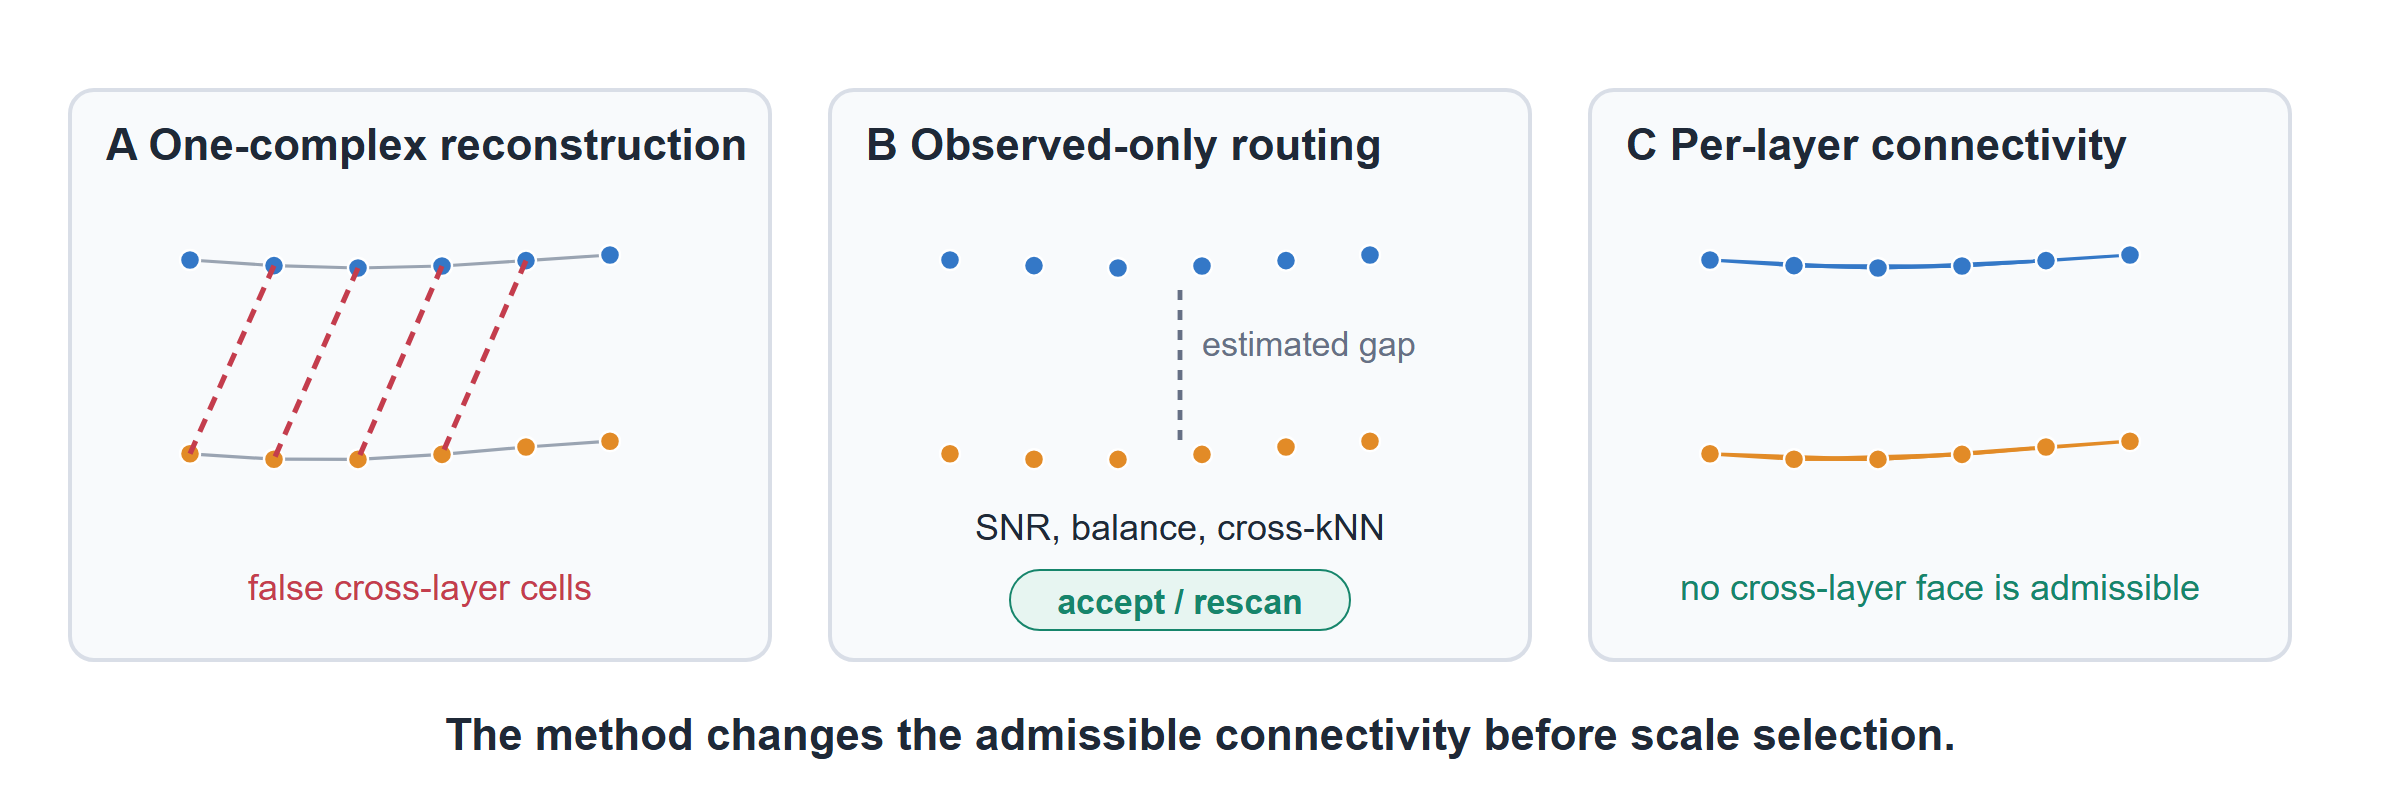
\includegraphics[width=\textwidth]{two_layer_workflow.png}
  \caption{Two-layer 전환의 핵심. 하나의 3D complex(A)는 가까운 두 층 사이에
  거짓 연결을 만들 수 있다. 관측 좌표만으로 분리 가능성과 sampling을 검사하고(B),
  통과한 경우 각 층 안에서만 연결하면 cross-layer face는 애초에 후보가 아니다(C).}
\end{figure}

\subsection{알고리즘을 네 단계로 읽기}

\paragraph{1단계: 공통 방향을 찾는다.}
각 점 주변의 이웃 12개로 작은 평면의 법선\footnote{법선(normal)은 표면에 수직인
화살표다. 바닥의 법선은 위아래 방향, 벽의 법선은 옆 방향이다.}을 구한다.
법선은 앞뒤 부호가 바뀔 수 있으므로 단순 평균 대신 orientation tensor를 써서
두 표면이 공통으로 ``위아래''라고 말하는 방향을 찾는다.

\paragraph{2단계: 높이를 따라 두 무리로 나눈다.}
각 점을 공통 법선 방향에 투영하면 높이 $h_i$가 생긴다. 낮은 모드와 높은 모드로
결정론적 two-means 분리를 한다. 두 표면이 함께 완만하게 휜 합성 조건에서는
공통 quadratic trend $q(u,v)$를 먼저 빼고 남은 높이로 나눌 수 있다.

\paragraph{3단계: 자신 없으면 결과를 내지 않는다.}
다음 세 관측량을 본다.

\begin{itemize}
  \item 작은 층도 전체 점의 20\% 이상인가?
  \item 두 층 중심의 간격이 각 층의 흔들림보다 충분히 큰가? 최종 합성 protocol의
  SNR 기준은 3.0이다.
  \item 가까운 이웃들이 다른 층으로 자주 섞이지 않는가? cross-kNN 비율 기준은
  0.05 이하다.
\end{itemize}

통과하지 못하면 억지 표면을 내지 않고 다음 중 하나로 끝낸다.
\begin{itemize}
  \item \code{unsupported}: 두 층 자체를 믿을 수 없음,
  \item \code{rescan\_required}: 층은 보이지만 sampling이 부족함,
  \item \code{algorithm\_failure}: 만든 메시가 약속한 구조를 어김.
\end{itemize}
이것이 \textbf{fail-closed}\footnote{Fail-closed는 애매할 때 성공이라고 우기지 않고
안전한 실패 상태로 닫는 설계다. 의료·제조·자율 시스템처럼 잘못된 성공이 위험한
곳에서 중요하다.}다.

\paragraph{4단계: 층마다 따로 삼각분할한다.}
각 층을 자기 접평면에 투영해 2D Delaunay 삼각분할을 하고, 다시 3D 점 번호로
돌린다. 이를 짧게 쓰면

\begin{equation}
\mathcal{T}_{\mathrm{layer}}
=\mathcal{D}_2(\Pi_0X_0)\cup\mathcal{D}_2(\Pi_1X_1),
\qquad X_0\cap X_1=\varnothing.
\end{equation}

고등학생식으로 읽으면 ``0번 층에서 만든 삼각형과 1번 층에서 만든 삼각형을
합친다. 두 층을 가로지르는 삼각형은 만들지 않는다''는 뜻이다.

\section{실험을 믿을 수 있게 만든 장치}

\subsection{동결 protocol}

결과를 본 다음 기준을 바꾸면 시험 문제를 보고 답안지를 고치는 것과 같다.
이 프로젝트는 parameter, gate, 비교 방법, 평가값을 먼저 고정하고 새로운
held-out panel을 한 번만 열었다. 이를 frozen 또는 preregistered test라고 부른다.

\subsection{정보 경계}

후보 방법은 결합된 관측 XYZ만 받는다. 정답 layer label과 dense reference는
채점할 때만 쓴다. S3DIS에서는 annotation으로 ``바닥-천장 평가 corpus''를
자동 추출하지만, 재구성 후보에는 floor/ceiling 이름이나 정답 층을 주지 않는다.
따라서 \textbf{corpus를 만드는 정보}와 \textbf{알고리즘이 판단하는 정보}를
구분해야 한다.

\subsection{평균만 보지 않는다}

평균 F-score가 높아도 몇 개 쉬운 사례가 전체 평균을 끌어올릴 수 있다.
그래서 각 사례에서 B5와 M1을 실제로 이겼는지 casewise win을 센다. 또한
topology error, false-safe, nonmanifold edge, subgroup coverage를 함께 본다.

\section{양성 결과 1: 144개 합성 확인 실험}

Phase 50은 결과를 보기 전에 고정한 새 패널이다. 점 수는 160 또는 256,
stress는 control, upper occlusion, 75:25 층 불균형, anisotropic noise,
sinusoidal common trend, local bump의 여섯 종류이고, 각각 12회 반복했다.
모든 사례는 서로 다른 proper 3D rotation을 받아 특정 좌표축에 기대지 못하게 했다.

\begin{table}[tbp]
\centering
\caption{Phase 50 합성 패널의 핵심 결과. F-score는 높을수록 좋고, geometry
loss와 topology error는 낮을수록 좋다.}
\small
\begin{tabularx}{\textwidth}{Xrrr}
\toprule
방법 & 평균 F-score & Geometry loss & Topology error \\
\midrule
Layer-first two-layer & \textbf{0.898536} & \textbf{0.126043} & \textbf{0} \\
B5 PCA-anisotropic alpha & 0.515603 & 0.140552 & 45,606 \\
M1 weighted power-alpha & 0.620140 & 0.137152 & 11,925 \\
\bottomrule
\end{tabularx}
\end{table}

후보는 144/144를 안전하게 수락했고 false-safe는 0이었다. B5와 M1 각각에
대해 144/144 사례에서 F-score가 더 높았다. Global-normal 기본 방법이 잘못
통과시킨 여섯 사례도 shared-trend 후보가 모두 고쳤다. 사전등록한 safety,
geometry, topology, ablation gate가 모두 통과했다.

이 결과는 강하지만 범위가 좁다. N은 160 이상이고, 공간 outlier가 없으며,
두 층이 전역적으로 분리 가능한 합성 표면에 대한 결과다.

\section{양성 결과 2: 다른 건물의 S3DIS 63개 방}

합성 데이터에서만 잘 되면 generator의 습관을 외운 것일 수 있다. 그래서
Stanford Large-Scale 3D Indoor Spaces(S3DIS)\footnote{S3DIS는 실제 건물의
실내 공간을 3D point cloud로 제공하는 공개 연구 데이터다. I. Armeni et al.,
``3D Semantic Parsing of Large-Scale Indoor Spaces,'' CVPR, 2016.}를 사용했다.

Areas 1, 2, 3, 4, 6으로 eligibility와 추출 규칙을 보정하고, 다른 건물인
Area 5는 protocol과 evaluator를 commit한 뒤 한 번만 열었다. 고정된 자동 규칙이
63개 floor-ceiling 방을 선택했다. 수동으로 좋은 방만 골라 넣거나 나쁜 방을
빼지 않았다.

\begin{table}[tbp]
\centering
\caption{Phase 51C S3DIS Area-5 결과.}
\small
\begin{tabularx}{\textwidth}{Xrrr}
\toprule
방법 & 평균 F-score & Geometry loss & Topology error \\
\midrule
Layer-first two-layer & \textbf{0.805611} & \textbf{0.116385} & \textbf{0} \\
B5 PCA-anisotropic alpha & 0.420983 & 0.243356 & 5,214 \\
M1 weighted power-alpha & 0.323764 & 0.228920 & 13,375 \\
\bottomrule
\end{tabularx}
\end{table}

후보는 62/63 방을 안전하게 수락했고 false-safe는 0이었다. 유일한
\code{rescan\_required}인 hallway 5도 실제 topology는 안전했고 F-score가
0.989640이었다. B5와 M1 모두 63개 방에서 계산 가능했으며, 후보는 각각에 대해
63/63 casewise win을 기록했다.

중요한 ablation이 있다. S3DIS에서는 더 단순한 global-normal 모델이
shared-trend 모델과 표시 정밀도에서 같은 평균 F-score와 같은 62/63 coverage를
보였다. 따라서 real positive result를 shared-trend의 우월성으로 설명하면 안 된다.

\begin{figure}[tbp]
  \centering
  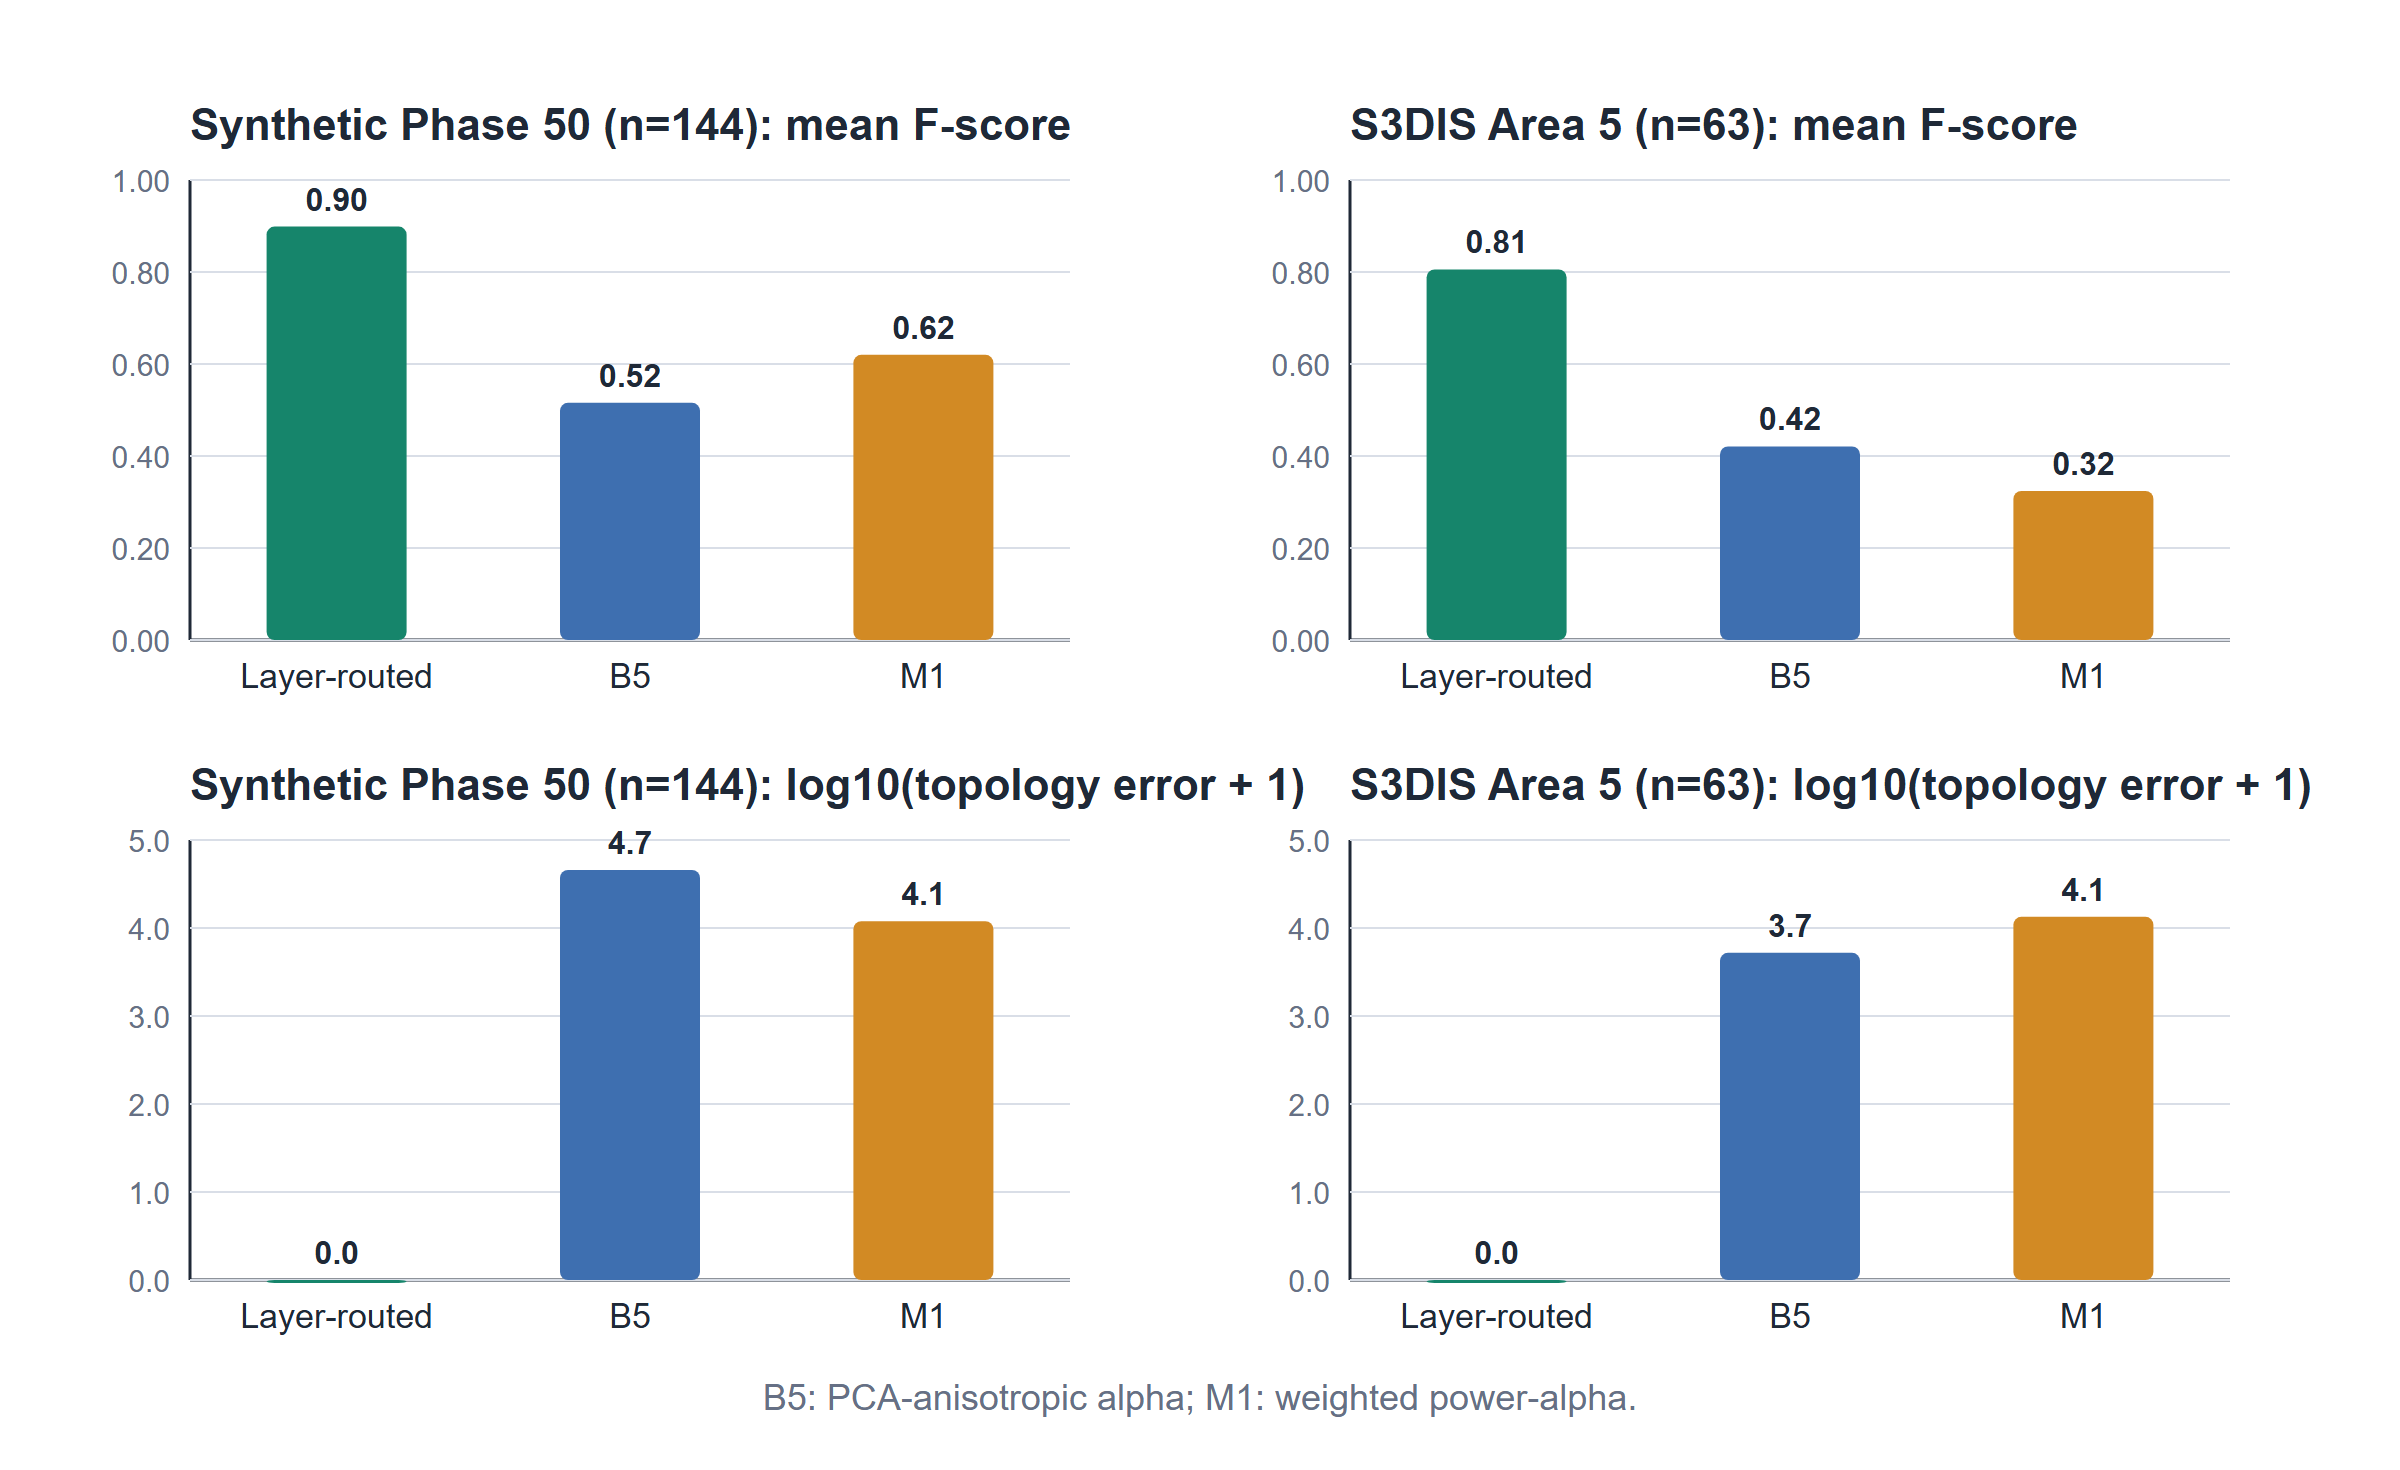
\includegraphics[width=\textwidth]{two_layer_results.png}
  \caption{두 확인 패널의 요약. 위쪽은 평균 F-score, 아래쪽은 표시를 위해
  $\log_{10}(\mathrm{topology\ error}+1)$를 쓴 값이다. 정확한 raw total은
  본문의 표에 있다.}
\end{figure}

\section{왜 이것이 positive paper가 될 수 있는가?}

처음 질문은 ``PFTF로 $\alpha$를 더 잘 찾을 수 있는가?''였다. 그 답은 현재
증거에서 부정적이다. 그러나 연구 도중 더 정확한 문제가 발견되었다.

\begin{quote}
두 층 사이의 거짓 연결은 잘못 고른 숫자 하나의 문제가 아니라,
허용 가능한 연결 집합을 잘못 정의한 문제다.
\end{quote}

Layer-first 방법은 비교 방법의 점수만 조금 조정하지 않는다. 가설 공간 자체를
바꾼다. B5는 local metric을 바꾸고 M1은 regular triangulation을 바꾸지만,
둘 다 두 표면의 합집합을 하나의 3D complex로 처리한다. Layer-first는 관측 가능한
두 층이라는 구조를 이용해 문제를 두 개의 planar reconstruction으로 나눈다.

따라서 positive novelty는 다음 세 요소의 결합이다.

\begin{enumerate}
  \item 정답 label 없이 관측 좌표로 두 층을 추론한다.
  \item 분리가 불확실하거나 sampling이 부족하면 fail-closed한다.
  \item 통과한 경우 cross-layer 연결을 구성 공간에서 제거한다.
\end{enumerate}

이 결론은 PFTF 이름을 억지로 붙여 얻은 것이 아니다. 오히려 강한 음성 결과를
인정하고 구조적 문제로 초점을 옮겼기 때문에 얻었다. 프로젝트 이름은 연구의
출발점을 보여 주지만, 최종 positive claim의 주인공은 observed-only routing과
constrained connectivity다.

\section{무엇까지 말할 수 있고, 무엇은 아직 말하면 안 되는가?}

\begin{table}[tbp]
\centering
\caption{현재 근거의 경계.}
\small
\begin{tabularx}{\textwidth}{p{0.46\textwidth}p{0.46\textwidth}}
\toprule
\multicolumn{1}{c}{\textbf{말할 수 있음}} &
\multicolumn{1}{c}{\textbf{아직 말하면 안 됨}} \\
\midrule
충분히 planar하고 넓게 겹치며 간격이 큰 두 층에서 양성 결과 &
가까이 붙고 서로 가려지는 wall-board 층으로의 전이 \\
N=160/256 non-outlier 합성 panel에서 144/144 안전 수락 &
N<160의 sparse sampling이나 임의 spatial outlier에 대한 안전성 \\
S3DIS Area-5 floor-ceiling 63개 방의 building-disjoint held-out 검증 &
교차 표면, 임의 multi-surface scene, 복잡한 boundary의 일반 해법 \\
관측 XYZ만을 이용한 reconstruction routing &
semantic floor/ceiling pair의 자동 발견 \\
B5/M1 대비 geometry와 topology 우위 &
PFTF/local-SPD 또는 shared-trend 자체의 우월성 \\
동일 실행의 결정론적 재현과 frozen gate 통과 &
exact geometric predicate, runtime/memory 우위, production deployment \\
\bottomrule
\end{tabularx}
\end{table}

또한 층별 2D Delaunay는 한 층 안의 큰 구멍을 가로지를 수 있다. 현재 방법은
boundary recovery를 포함하지 않는다. 향후에는 visibility-aware support,
boundary-aware planar meshing 또는 layer 내부 alpha restriction, 자동 pair
discovery, 센서별 artifact, exact predicate를 따로 검증해야 한다.

\section{대학원생이 이 연구에서 배울 수 있는 것}

\subsection{복잡한 모델보다 맞는 문제 정의가 먼저다}

좋은 $\alpha$를 찾는 일을 아무리 정교하게 해도, 애초에 허용하면 안 되는 연결이
후보 집합에 들어 있으면 해결이 어렵다. Parameter tuning 전에 가설 공간이 물리적
구조와 맞는지 확인해야 한다.

\subsection{``구성 가능''과 ``성능이 좋음''을 구분하라}

Phase 47의 analytic spatial-SPD complex는 수학적으로 일관됐다. Phase 48의
PFTF 예측 변환도 모두 invertibility audit를 통과했다. 그러나 성능 gate는 실패했다.
정리, 구현, 수치 안정성, 예측력, 실제 효용은 서로 다른 증거를 요구한다.

\subsection{Negative result는 다음 가설의 지도다}

PFTF/local-SPD가 B5를 이기지 못했다는 결과를 숨겼다면, 연구는 계속 더 복잡한
metric을 튜닝했을 가능성이 크다. 음성 결과를 정확히 기록했기 때문에 ``scale이
아니라 connectivity''라는 더 좋은 질문으로 이동할 수 있었다.

\subsection{Held-out discipline은 알고리즘의 일부다}

새 데이터에서 수치가 나빠질 때마다 gate를 바꾸면 어떤 방법도 좋아 보이게 만들 수
있다. Protocol commit, 한 번만 여는 held-out, casewise win, false-safe 0 같은
절차는 부가 문서가 아니라 주장의 신뢰도를 만드는 핵심 설계다.

\subsection{큰 수치보다 좁고 재현 가능한 문장이 강하다}

``모든 alpha-shape 문제를 해결했다''는 문장은 현재 증거보다 크다. 반면
``서로 식별 가능한 long-gap two-layer에서 층별 재구성이 두 frozen alpha
comparator보다 우수했다''는 문장은 좁지만 반증 가능하고 재현 가능하다.
논문에서 강한 주장은 넓은 문장이 아니라, 근거와 정확히 맞는 문장이다.

\section{저장소를 읽는 가장 짧은 순서}

프로젝트를 직접 확인하려면 다음 순서가 가장 쉽다.

\begin{enumerate}
  \item \code{README.md}: 현재 지원되는 주장과 지원되지 않는 주장을 먼저 본다.
  \item \code{docs/PFTF\_ALPHA\_CLAIM\_EVIDENCE.md}: 주장-근거-경계 표를 본다.
  \item \code{docs/TWO\_LAYER\_CONFIRMATORY\_RESULT\_PHASE50.md}: 144개 합성
  확인 실험을 본다.
  \item \code{docs/S3DIS\_ROOM\_LAYER\_VALIDATION\_RESULT\_PHASE51C.md}:
  real held-out 결과를 본다.
  \item \code{draft/paper\_kr.tex}: 논문 수준의 방법, 실험, 토론을 읽는다.
\end{enumerate}

Phase 50의 재현 명령은 다음과 같다.

\begin{verbatim}
.\.venv\Scripts\python.exe -m pftf_alpha.two_layer_confirmatory `
  --output benchmark-out\two_layer_confirmatory_phase50.json
\end{verbatim}

S3DIS 실험은 공개 데이터이지만 매우 큰 archive와 frozen extraction protocol이
필요하다. 결과를 다시 계산할 때는 결과 JSON만 보고 코드를 튜닝하지 말고,
protocol·calibration·Area-5 information boundary를 그대로 보존해야 한다.

\section{용어를 다시 한 번 쉽게 정리하기}

\begin{description}
  \item[점군(point cloud)] 3D 공간에 흩어진 좌표들의 모임.
  \item[Convex hull] 점군을 팽팽한 고무막으로 감싼 가장 작은 볼록 껍질.
  \item[Alpha complex / alpha shape] Delaunay 연결 중 scale 기준을 통과한
  cell의 집합과 그 경계.
  \item[$\alpha$] 어느 scale까지 연결을 허용할지 정하는 손잡이.
  \item[Anisotropic metric] 방향마다 거리를 다르게 재는 자.
  \item[SPD] 그 방향 자가 뒤집히지 않게 하는 행렬 조건.
  \item[Topology] 표면의 연결 성분, 구멍, 다리처럼 ``찢고 붙이지 않고는
  바뀌지 않는'' 구조.
  \item[False bridge] 원래 떨어진 두 표면을 잘못 잇는 edge/face/cell.
  \item[Fail-closed] 불확실할 때 성공 결과를 내지 않고 안전 상태로 닫는 것.
  \item[Held-out] 개발 중 보지 않고 마지막 검증에만 쓰는 시험 데이터.
  \item[Casewise win] 평균이 아니라 각 사례마다 비교 방법을 이겼는지 세는 것.
  \item[Ablation] 방법의 한 부분을 빼거나 단순화해, 실제로 무엇이 효과를 냈는지
  확인하는 시험.
\end{description}

\section*{한 페이지 요약}
\addcontentsline{toc}{section}{한 페이지 요약}

Alpha shape은 convex hull보다 오목한 경계와 분리된 부품을 잘 나타내지만,
$\alpha$가 작으면 구멍이 나고 크면 떨어진 표면이 붙는다. PFTF-alpha 프로젝트는
처음에 PFTF의 방향 관계를 local-SPD 거리나 좌표 변환으로 바꾸어 더 좋은
alpha complex를 만들 수 있는지 시험했다. 전역 affine-SPD와 한 analytic
quadratic-shear map에서는 일관된 complex를 만들 수 있었지만, 임의 local-SPD,
PFTF-conditioned map, reconstruction 성능 우위는 지지되지 않았다. Real held-out
점군에서도 강한 B5 anisotropic alpha가 PFTF 후보보다 좋았다.

연구의 전환점은 서로 분리된 두 표면에서 거짓 다리의 원인이 scale만이 아니라
연결 허용 규칙이라는 사실이었다. 새 방법은 관측 XYZ로 두 층을 추론하고,
분리와 sampling이 충분한지 검사해, 자신 없으면 fail-closed한다. 통과한 경우
각 층을 접평면에 투영해 별도의 2D Delaunay surface를 만들므로 cross-layer
face는 처음부터 존재할 수 없다.

동결된 144개 합성 확인 사례에서 후보의 평균 F-score는 0.898536으로 B5의
0.515603과 M1의 0.620140보다 높았고, 두 비교 방법 각각에 대해 144/144
casewise win과 topology error 0을 기록했다. 서로 다른 건물의 S3DIS Area-5
63개 floor-ceiling 방에서는 평균 F-score 0.805611, 63/63 win, topology error
0, safe accept 62/63, false-safe 0이었다. 모든 사전등록 gate가 통과했다.

최종 결론은 좁지만 긍정적이다. 충분히 평면적이고 넓게 겹치며 간격이 큰 두 층이
관측 좌표에서 식별 가능할 때, $\alpha$를 계속 조정하는 것보다 두 층을 먼저
분리하고 허용 가능한 연결을 제한하는 편이 더 정확하고 topology도 안전하다.
이 결과는 PFTF/local-SPD 또는 shared-trend의 우월성, 가까운 층, outlier,
임의 multi-surface, 자동 semantic 추출, exactness, deployment까지 지지하지는
않는다.

\section*{참고문헌과 근거 문서}
\addcontentsline{toc}{section}{참고문헌과 근거 문서}

\begin{enumerate}
  \item H. Edelsbrunner and E. P. M\"ucke, ``Three-Dimensional Alpha
  Shapes,'' \emph{ACM Transactions on Graphics}, 13(1), 43--72, 1994.
  \item H. Edelsbrunner, ``Weighted Alpha Shapes,'' Technical Report
  UIUCDCS-R-92-1760, University of Illinois at Urbana-Champaign, 1992.
  \item M. Teichmann and M. Capps, ``Surface Reconstruction with Anisotropic
  Density-Scaled Alpha Shapes,'' \emph{IEEE Visualization '98}, 67--72, 1998.
  \item I. Armeni et al., ``3D Semantic Parsing of Large-Scale Indoor
  Spaces,'' \emph{CVPR}, 1534--1543, 2016.
  \item 프로젝트 내부 근거 문서:
  \par
  \path{docs/PFTF_ALPHA_CLAIM_EVIDENCE.md},
  \path{docs/TWO_LAYER_CONFIRMATORY_RESULT_PHASE50.md},
  \path{docs/S3DIS_ROOM_LAYER_VALIDATION_RESULT_PHASE51C.md}.
\end{enumerate}

\end{document}
